\documentclass[12pt,a4paper,article,english,firamath]{nsi}
\pagestyle{empty}
\begin{document}
\titre{Exercises 01}
\classe{Euro 1\ere}
\maketitle


\begin{exercice}[]
    \picright{0.2}{img/missing_number}{Can you find the missing number (there are two ways to find it) ?}
\end{exercice}


\begin{exercice}[]
    \begin{center}
        \textit{
        As defined by the International Astronomical Union (IAU), the light-year is the product of the Julian year (365.25 days) and the speed of light (299,792,458 m/s).}
    \end{center}
    \begin{enumerate}
        \item How many kilometers is a light-year ?
        \item Give an order of magnitude of this distance.
    \end{enumerate}
\end{exercice}

\begin{exercice}[]
    \picleft{0.3}{img/parking}{Can you find the number of the parking spot covered by the car ?}
\end{exercice}

\begin{exercice}
    \picright{0.4}{img/cat_table_turtle}{How tall is the table ?}

\end{exercice}

\begin{exercice}[]
\begin{center}
    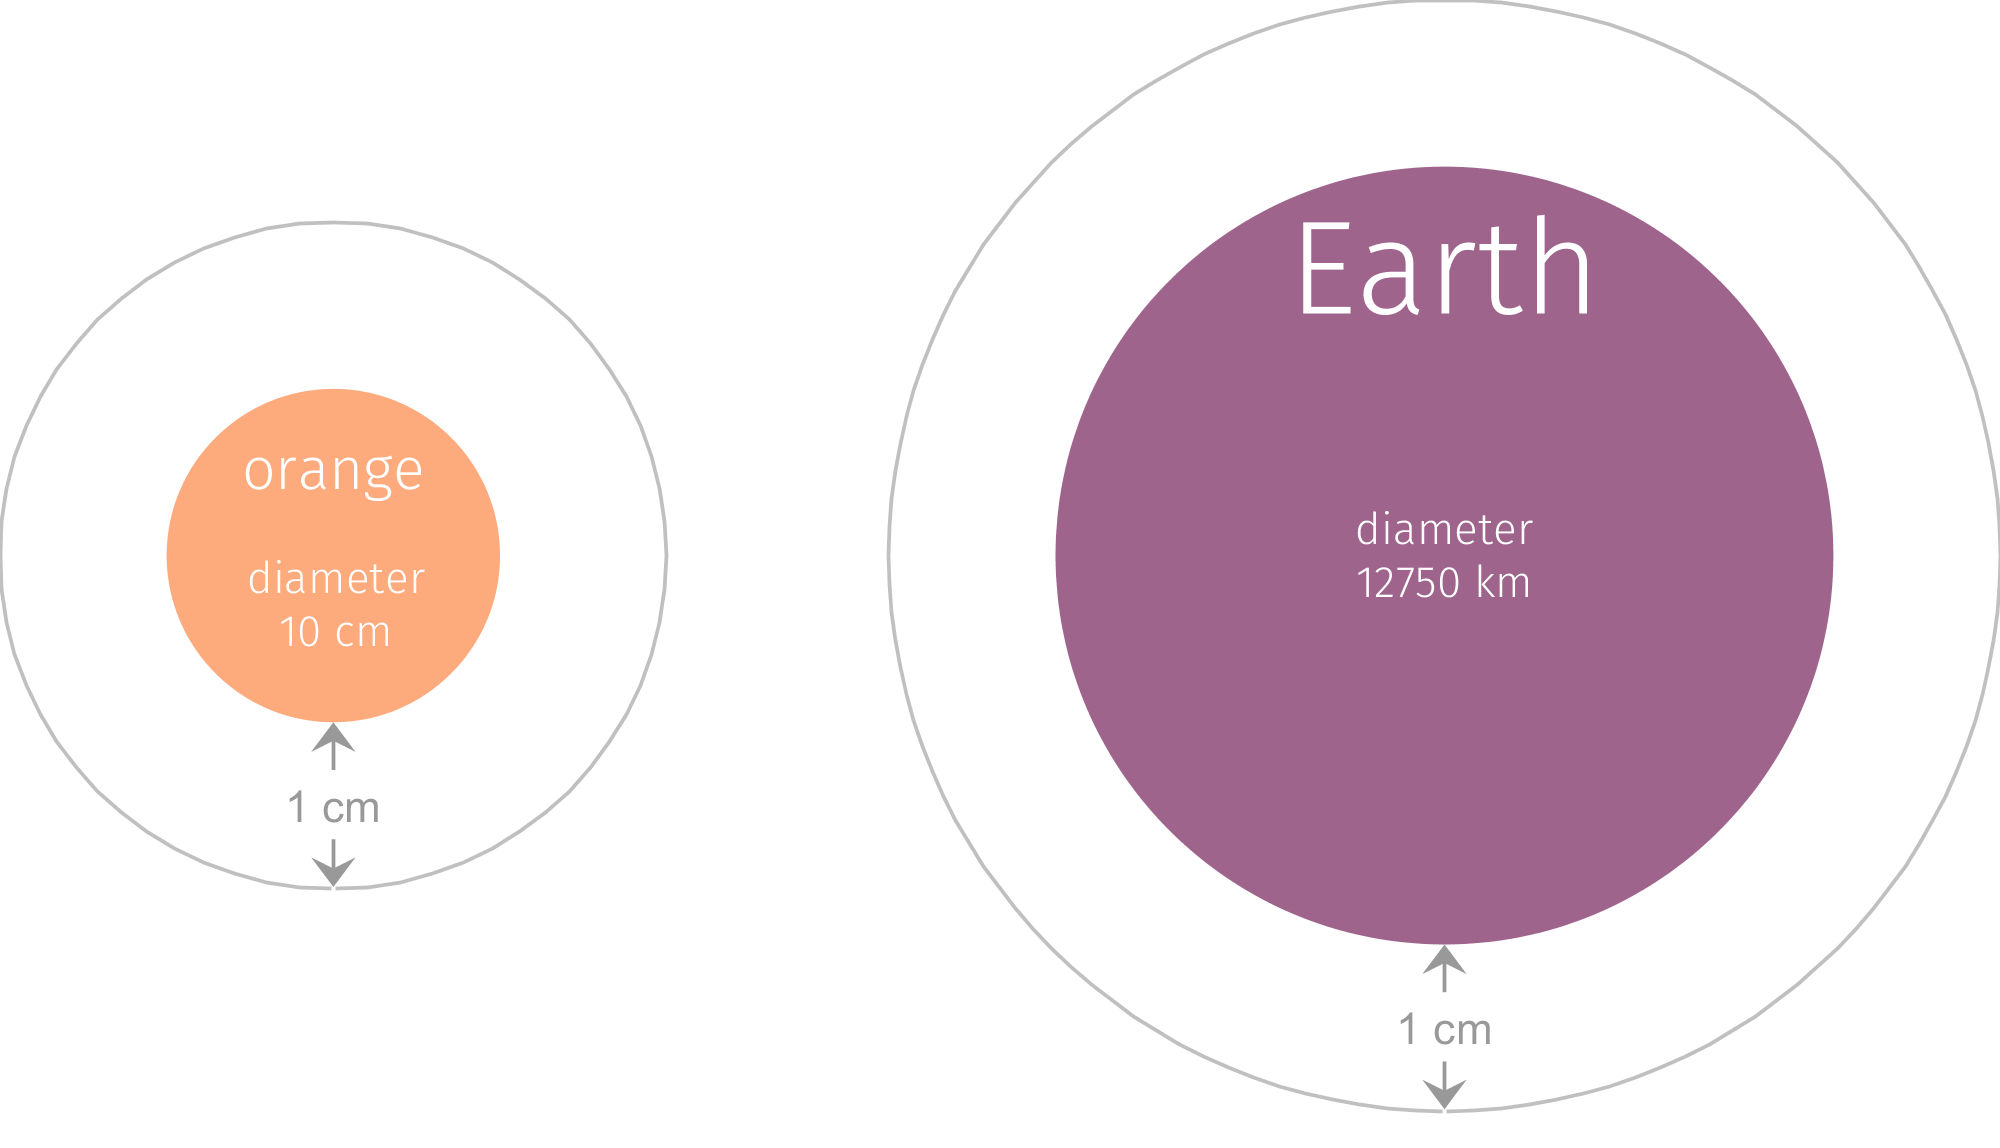
\includegraphics[width=9cm]{img/orange_and_earth.png}
\end{center}
\begin{enumerate}
    \item Consider a rope just long enough to make a full circle around the circumference of an orange (which can be considered as a sphere with a diameter of 10 cm). How much do we have to add to the rope's length so that it "floats" 1 cm above the surface of the orange ?
    \item Same question, replacing the orange with the Earth (which is much bigger, with a diameter of 12,750 km).
\end{enumerate}
\end{exercice}

\end{document}